\chapter{Background and Concepts}
In this chapter, we will introduce several main concepts related to our study.
\section{Agile software development}
\label{agile}
The term "Agile" represents the fast adaptation and response to the changes.\cite{WhatisAg98:online}
Agile software development is a new method of software development that implements the ideology of "agile". Agile software development advocates the continuous development of software teams. The software development under this methodology will have shorter planning/development time before it delivers to the costumers and could better adapt to changes in the environment and requirements.
\par
Agile software development uses an iterative way in the development process. The traditional software development process, like the waterfall method, requires the long and complicated planning process, and a complicated document. Once one phase of the development is done, the teams shouldn't change the output (document and code) of this phase.\cite{cusumano1995beyond} In contrast, the agile software development aims to satisfy the customer with early and continuous delivery of the software.\cite{beck2001manifesto}. Early means the shorter time before software delivery. Continuous means the development does not end with the delivery. Delivery means the end an iteration, together with a demonstration to stakeholders. After delivery, the team continue to next iteration according to the feedback it gets from stakeholders. In each iteration, the team not aims to add major features to the software, rather their goal is to have a working and deliverable release\cite{beck1999embracing}. In the ideology of agile, the best design the software product comes from the iterative development, rather than the tedious planning.\cite{beck2001manifesto}
\par
The rapid development doesn't mean low software development quality. On the contrast, the quality of software design is highly appreciated in the agile software development. The automatic testing is widely used in Agile. The test cases will be defined and implements from the beginning of the development process. The testing goes through the whole development iteration ensure the software has a high enough quality to be released or demonstrate to costumers at any point of an iteration\cite{Agilesof32:online}.
\par
The agile software development processes include collaboration across different groups, ie. bushiness development team, software development team, test team, and costumers. It values more face to face communications\cite{beck2001principles} and feedbacks. The goal for these communications is, firstly to let everyone in the multifunctional agile team understand the whole project, secondly, to receive feedback that helps the software in the right development track that aligns with the requirement of the stakeholders. \cite{beck2001manifesto} 
\par
According to the Manifesto for Agile Software Development, compared with traditional software development, the agile software development value these aspects: \cite{beck2001manifesto}
\begin{itemize}
\item Individuals and interactions over processes and tools.
\item Working software over comprehensive documentation.
\item Customer collaboration over contract negotiation.
\item Responding to change over following a plan.
\end{itemize}
\section{CI/CD}
In the software development, CI/CD refers to continuous integration, continuous delivery and continuous deployment.\cite{Continuo67:online}. As we mentioned in \ref{agile}, agile software development requires continuous software quality assurance and iterative development. Currently, CI/CD is one set of the necessary practices for the team to become agile by achieving the requirements above. Figure \ref{fig:cicd} shows the relationship between these 3 practices.
\begin{figure}[h]
    \centering
    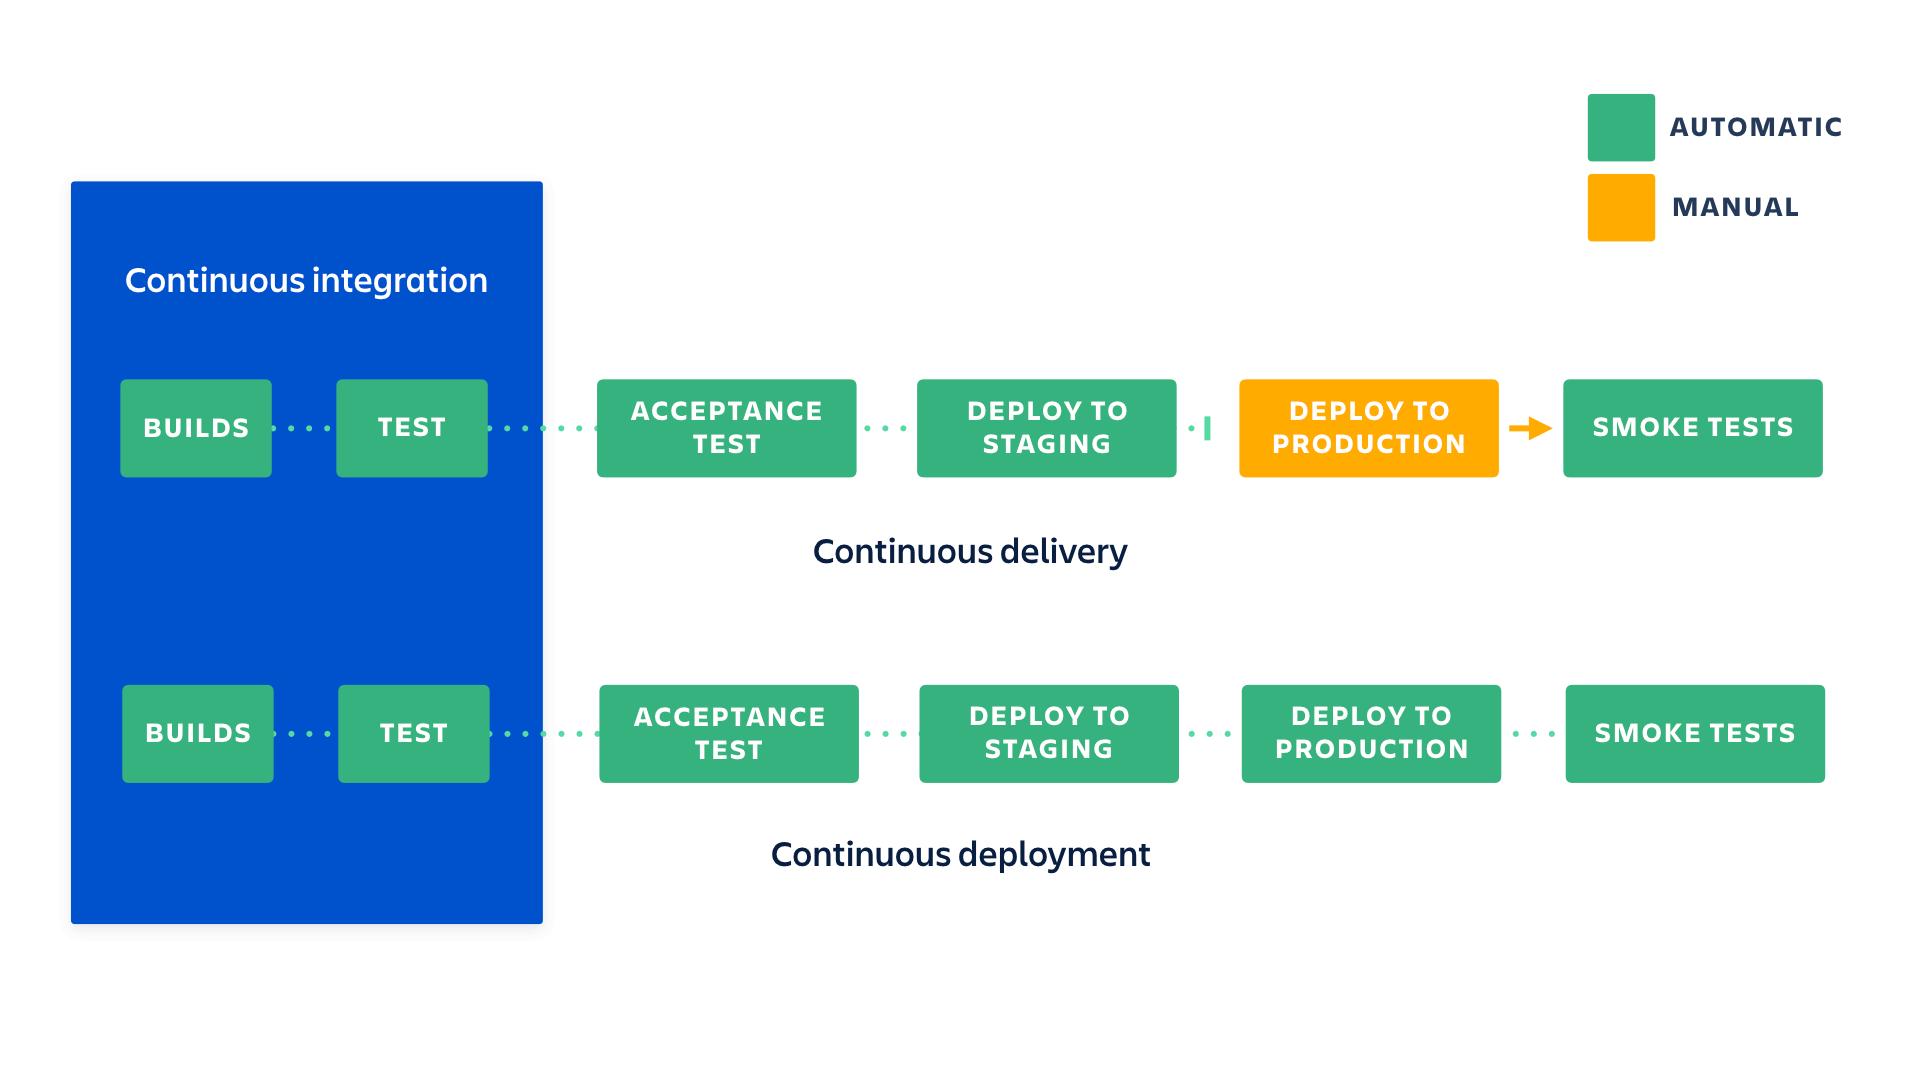
\includegraphics[width=0.95\textwidth]{pics/cicd.png}
    \caption{The relationship between continuous integration, continuous delivery and continuous deployment}
    \label{fig:cicd}
\end{figure}
\subsection{Continuous Integration}
Continuous interaction is the base practice of all practices within CI/CD, and continuous delivery/deployment is based on the continuous interaction.\cite{Continuo67:online}
The continuous integration means the team integrate each team member's work into main codebase frequently(multiple times per day). "Integrate" means merge the code to the main codebase.\cite{fowler2006continuous}. The continuous interaction rely on 2 practices: \textit{Build Automation} and  \textit{Test Automation}. The definition of these 2 practices are:
\begin{itemize}
    \item \textit{Test Automation:} Test automation means using separate software to execute the software automated, without human intervention. It could help the team to test fast and test early. \cite{Testauto48:online}
    \item \textit{Build Automation:} Automate the process of creating software build. This means to automate the dependency configuration, source code compiling, packaging and testing. It is viewed as the first step to continuous integration\cite{Buildaut62:online}
\end{itemize}
With the help of these 2 practices, for each developer in the team, the workflow in continuous interaction as follows:\cite{fowler2006continuous} In the development of each feature, the developer first pull the code from the main codebase. During the development, new test cases could also be added to the automated test. After the development is done, automated testing also runs on the code to maintain the code quality and minimize the number of bugs from the beginning. The build automation compiled the code locally in the development machine. 
\par
After the step above, the developer already has the executable and the high quality (passed the automated test) code in the development machine before submitting the change to the code base. This represents the principle of quality and automation in agile software development. In the next step, the developer commits changes to the repository, which is the main codebase, and the system check the conflict and do the test/build again, to make sure that there are not any bugs missed in the test on the development machine.
If the code passes this build and test, it will be merged to the main codebase and the integration is done.
\subsection{Continuous Delivery and Continuous Deployment}
Continuous delivery is practices that software development team build a software that can be released at any time of the lifecycle.\cite{fowler2013continuous}This means the software always maintains a high quality and in a deployable state.\cite{WhatisCo47:online} It is a subset of agile, which focuses on the software delivery.\cite{Continuo97:online} From the last section, we introduce the concept of continuous interaction. The continuous delivery is based on continuous interaction but further automate the software deployment pipeline. In the software deployment pipeline, the team divide build into several stages, first build the product and then push the product into the production-like environment for further testing. This ensures that the software could be pushed to production at any time. However, in continuous delivery, the deployment of software into production is done manually.
The benefit of continuous delivery includes:\cite{WhatisCo47:online}\cite{fowler2013continuous}
\begin{itemize}
    \item High code quality: The automate and continuous testing ensure the quality of the software.
    \item Low risk: The software could be related at any time, and it's easier to release and harder to make the mistake
    \item Short time before going to the market: The iteration of software development is much shorter. The automation in testing, deployment, environment confirmation included in the process, and the always read-to-deploy status shorten the time from development to market.
\end{itemize}
The continuous deployment is based on continuous delivery. The only difference is continuous deployment automates the deployment process. In continuous delivery, the software is deployable but not deploy without manual approval. In the continuous deployment, each change that passed automated build and testing will be deployed directly. The continuous deployment is a relatively new concept that most company not yet put the practice into production.\cite{leppanen2015highways} While continuous delivery is the required practice for the company to be DevOps and it is already being widely used.
\section{DevOps}
\begin{quotation}
    The fundamental goal of DevOps is to minimize the service overhead so that it can response to change with minimal effort and deliver maximum amount of value during its lifetime.
    \begin{flushright}
        -- Markus Suonto, Senior DevOps Consultant, Eficode
    \end{flushright}
\end{quotation}
\subsection{Definition}
DevOps is a set of practices that aims to combine different, traditionally separated disciplines (eg. software development, operations, QA, and others) in cross-functional teams with the help of automation of work in order to speed up software delivery without risking high quality.\cite{bass2015devops}
\par
DevOps is the extension and evolution\cite{lwakatare2016relationship}\cite{leite2019survey} of Agile. DevOps and Agile both driven by the collaboration ideology and the adoption of DevOps needs Agile as the key factor.\cite{lwakatare2016relationship} In the pre-DevOps era, the Development and Operation are two different teams with difference goal.  The interface between them is based on the ticket system which the operation team do the ticket management. As we mentioned at \ref{agile}, the goal of Agile is to shorten the deliver life cycle and delivery software quickly to the costumers. So when practice agile development method under this scenario, the development try to to deliver the code they develop earlier but the operation team usually will delay the process for quality control or other reasons. In practice, this causes the delay between the code change and the software delivery to the costumers\cite{leite2019survey}. 
\par
The lack of communication and conflict between developers and operation team slow down the software delivery process and also make it harder for the teams to be real Agile. Thus the concept "DevOps" is being proposed at 2008, for eliminating of the boundary between developers (Dev) and operation team (Ops) and enhance the collaboration within an organization.
\subsection{DevOps Practices}
